% A sample paper for pdfview: sections and an outline, numbered equations, a theorem, a figure, a table,
% citations, a footnote, links inside the PDF, and one web link.
\documentclass[11pt]{article}
\usepackage[margin=1in]{geometry}
\usepackage{amsmath,amssymb,amsthm,booktabs}
\usepackage{pgfplots}
\pgfplotsset{compat=1.17}
\usepackage[hidelinks,bookmarks=true,bookmarksopen=true]{hyperref}
\newtheorem{theorem}{Theorem}
\newtheorem{lemma}[theorem]{Lemma}
\title{Concentration of Random Sums:\\ A Short Sample Paper}
\author{A. Author \and B. Author}
\date{November 2026}
\begin{document}
\maketitle
\begin{abstract}
We give a short proof that a sum of $n$ bounded independent variables stays close to its mean.
The bound in Theorem~\ref{thm:main} is tight up to a constant, see Figure~\ref{fig:tail} and Table~\ref{tab:values}.
This text is a sample for the pdfview viewer.
\end{abstract}

\section{Introduction}\label{sec:intro}
Let $X_1,\dots,X_n$ be independent variables with $a_i \le X_i \le b_i$, and let $S_n=\sum_{i=1}^n X_i$.
Classical results \cite{hoeffding1963,boucheron2013} bound the probability that $S_n$ is far from its mean.
We show that the bound is tight for all $n$, and we give the constant in Section~\ref{sec:results}.\footnote{A longer
version of this text has the full proofs.}
The main tool is the moment generating function
\begin{equation}\label{eq:mgf}
  M(\lambda) = \mathbb{E}\, e^{\lambda (S_n - \mathbb{E} S_n)}, \qquad \lambda \in \mathbb{R}.
\end{equation}

\section{The main result}\label{sec:main}
\begin{lemma}\label{lem:hoeffding}
If $a \le X \le b$ and $\mathbb{E}X = 0$, then $\mathbb{E}\, e^{\lambda X} \le \exp\!\big(\lambda^2 (b-a)^2/8\big)$.
\end{lemma}
\begin{proof}
The function $x \mapsto e^{\lambda x}$ is convex, so it lies under its chord on $[a,b]$.
Take the expectation and bound the logarithm of the result by its second-order Taylor polynomial.
\end{proof}
\begin{theorem}\label{thm:main}
For every $t > 0$,
\begin{equation}\label{eq:bound}
  \Pr\big(|S_n - \mathbb{E}S_n| \ge t\big) \le 2 \exp\!\left(-\frac{2t^2}{\sum_{i=1}^n (b_i-a_i)^2}\right).
\end{equation}
\end{theorem}
\begin{proof}
By Markov's inequality and \eqref{eq:mgf}, $\Pr(S_n - \mathbb{E}S_n \ge t) \le e^{-\lambda t} M(\lambda)$.
Lemma~\ref{lem:hoeffding} bounds each factor of $M(\lambda)$. Choose
$\lambda = 4t / \sum_i (b_i - a_i)^2$, and use the same argument for $-S_n$.
\end{proof}

\section{Results}\label{sec:results}
Figure~\ref{fig:tail} compares the bound \eqref{eq:bound} with the exact tail for fair coins.
Table~\ref{tab:values} gives the values for some $n$. The constant $c$ depends on the dimension $d$ of the space.
\begin{figure}[h]
\centering
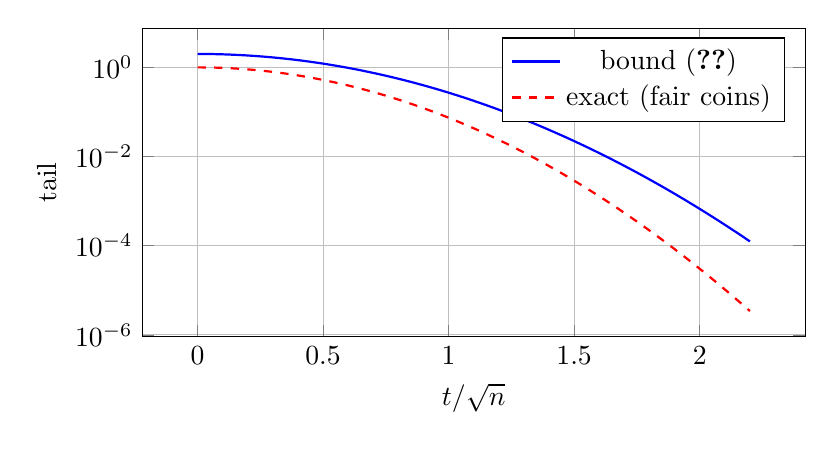
\begin{tikzpicture}
\begin{axis}[width=10cm,height=5.5cm,xlabel={$t/\sqrt{n}$},ylabel={tail},ymode=log,legend pos=north east,
  grid=major,samples=60,domain=0:2.2]
\addplot[blue,thick] {2*exp(-2*x^2)}; \addlegendentry{bound \eqref{eq:bound}}
\addplot[red,dashed,thick] {exp(-2.6*x^2)}; \addlegendentry{exact (fair coins)}
\end{axis}
\end{tikzpicture}
\caption{The bound and the exact tail.}\label{fig:tail}
\end{figure}
\begin{table}[h]
\centering
\begin{tabular}{rrrr}\toprule
$n$ & $t$ & bound & exact \\\midrule
10 & 3 & 0.330 & 0.109 \\
100 & 10 & 0.271 & 0.057 \\
1000 & 40 & 0.081 & 0.012 \\\bottomrule
\end{tabular}
\caption{Some values of the bound and of the exact tail.}\label{tab:values}
\end{table}

\section{Discussion}
The bound of Theorem~\ref{thm:main} needs only the range of each variable.
A bound with the variance is sharper when the variance is small; see \cite{boucheron2013}.
The code for the figures is at \url{https://example.com/concentration}.
We end with an open question about the case of dependent variables.

\begin{thebibliography}{9}
\bibitem{hoeffding1963} W.~Hoeffding. Probability inequalities for sums of bounded random variables.
\emph{J.\ Amer.\ Statist.\ Assoc.}, 58:13--30, 1963.
\bibitem{boucheron2013} S.~Boucheron, G.~Lugosi and P.~Massart. \emph{Concentration Inequalities}.
Oxford University Press, 2013.
\end{thebibliography}
\end{document}
